% Import the LaTeX style file and load some common packages
\documentclass[final]{siamart1116}
\usepackage{amsfonts}
\usepackage{amsopn}
\usepackage{listings}
\lstset{language=R}
\usepackage{xcolor}

% Declare the title, author, and any other front matter

% Title
\title{Environmental Tendencies of Salt Lake City}

% Authors: Full names and addresses
\author{Corbin Apple, Bridget Hyland, Ben Sterling}

% Page headers (visible after the cover page)
\headers{AMS 572 Group Project}{C. Apple, B. Hyland, B. Sterling}

% Start the document
\begin{document}
\maketitle

\section{Introduction}
It has been well established by The United States Environmental Protection Agency and other independent organizations that average temperature is increasing across the country. This study examines monthly temperature data from two stations: Rye Patch Dam, Nevada, and Salt Lake City International Airport, Utah. These stations were chosen because they are roughly at the same latitude ($40.498^{\circ}$N and $40.790^{\circ}$N), longitude ($118.316^{\circ}$W and $111.980^{\circ}$W), and elevation ($1260.3$m and $1287.8$m, for Rye Patch Dam and Salt Lake City respectively). Our data is from the National Centers for Environmental Information \cite{gsom_data}, which contains monthly data about major meteorological parameters at many locations across the country. We chose Salt Lake City and Rye Patch Dam because of their similar geographical characteristics. Data for Rye Patch Dam begins in 1935, but data for Salt Lake City only reaches back to 1948, so we used only years from 1948 to 2020 in our analysis. The dataset includes many parameters, but of particular interest to us were average temperature, average precipitation, number of days with thunderstorms, and total minutes of sunshine.

The goal of our first hypothesis is to examine whether the effects of climate change statistically differ between these two locations; if they do, we may be able to infer that the climate change is predominantly man-made. We accomplished this by calculating the monthly temperature anomaly at each location and comparing the mean temperature anomalies of the two locations. The goal of our second hypothesis is to determine predictors of temperature. We use a multiple linear regression with temperature as the response variable and precipitation, days with thunderstorms, and minutes of sunshine as the dependent variables.

\section{First Hypothesis}
Climate change is a well-documented phenomenon: on average, the global temperature is increasing. In this section, we test the hypothesis that temperature increases in Salt Lake City and Rye Patch Dam are not equal.

Temperature anomaly is used to compare change in temperature over time. A mean temperature is calculated over a long period of time, and this long-term mean is subtracted from more recent observations. For example, it is known that the global average temperature was $13.9^{\circ}$C between 1901 and 2000. If the global average temperature in 2015 was $14.5^{\circ}$C, then the temperature anomaly for that year would be $14.5 - 13.9 = 0.6^{\circ}$C. When analyzing temperature data over many years, it is advisable to use a temperature anomaly rather than absolute temperature because it eliminates seasonal variation within the year, allowing for a more significant result. This is an accepted and widely used method in climate analysis \textcolor{red}{[DOES THIS CITATION WORK??]} \cite{temp_anomaly}

The GSOM records the monthly average temperature at each location, so we determined temperature anomaly monthly. We calculated a January anomaly by averaging the January temperatures of each year from 1948 to 1974. Then, we subtracted this long-term mean from each January temperature from 1975 to 2020. We did the same for the other eleven months and for both locations, yielding different anomalies for each. In our data files, this is column CG, labeled TAVG ADJ. We used this anomaly in our comparison in place of the absolute temperature. It served to reduce the variance of each sample to produce a meaningful result.

Because of the large number of observations in each sample, we invoked the central limit theorem to approximate the distribution as normal. The Shapiro-Wilk test for normality gives a p-value of .01663 for the Salt Lake City sample and 0.0003392 for the Rye Patch Dam sample, which verifies that the normal approximation is appropriate ($P < 0.05$). The linear nature of the plots further supports our approximation.

Formally, our hypotheses are: $$ H_{0}: \mu_{SLC} = \mu_{RPD} \;\; vs. \;\; H_{a}: \mu_{SLC} \neq \mu_{RPD}.$$ Because the two stations have similar geographical characteristics (i.e. latitude, longitude, and elevation), we determined that this is an observational matched pairs analysis and used the paired t-test at $\alpha = 0.05$ accordingly. As such, it was not necessary to determine equality of variance between the two samples. We determined the test statistic to be $t = -16.46$. This is less than the critical value $-t_{n-1,\alpha/2} = -1.648$ (where n = 487). Also, the p-value is $2.2 \times 10^{-16}$, which is less than the significance level $\alpha = 0.05$. Based on these results, we reject $H_{0}$ and conclude that the mean temperature anomaly at Salt Lake City is significantly greater than the mean temperature anomaly at Rye Patch Dam. In other words, since 1975, the temperature has increased more at Salt Lake City than at Rye Patch Dam. The reason for this is not known, but previous research suggests that Salt Lake City emits a relatively large amount of carbon pollution per capita, which hastens the effects of climate change there \cite{obama_report}. These results, and useful statistics, are summarized in Tables \ref{tab:temp_diffs} and \ref{tab:t_test_results}.

\begin{table}[ht]
 \begin{centering}
 \begin{tabular}{|c|c c|} 
 \hline
 $$ & $\Delta T$ Salt Lake City & $\Delta T$ Rye Patch \\ [0.5ex] 
 \hline\hline
  $\mu$ & 1.1229 & 0.1317 \\ 
 \hline
 $\sigma$ & 1.9765 & 1.9226 \\
  \hline
 $n$ & 487 & 487 \\ 
  \hline
 $P_{Shapiro}$ & 0.0166 & 0.0003 \\ 
 \hline
 \end{tabular}
 \caption{Temperature Difference Statistics}
 \label{tab:temp_diffs}
 \end{centering}
\end{table}

\begin{table}[ht]
 \begin{centering}
 \begin{tabular}{|c|c|} 
 \hline
  $t$ & -16.46 \\ 
 \hline
 $df$ & 486 \\
  \hline
 $P$ & $2.2 \times 10^{-16}$ \\ 
  \hline
 Conf. Interval & $(-1.1095, -0.8728)$ \\ 
 \hline
 \end{tabular}
 \caption{Paired t Test Results for $\Delta T$}
 \label{tab:t_test_results}
 \end{centering}
\end{table}

We also present the Q-Q Plots in Figures \ref{fig:slc_diff_qqplot} and \ref{fig:rp_diff_qqplot} to visualize the data normality. The linear relationships suggest that both datasets are normal.

\begin{figure}
  \centering
  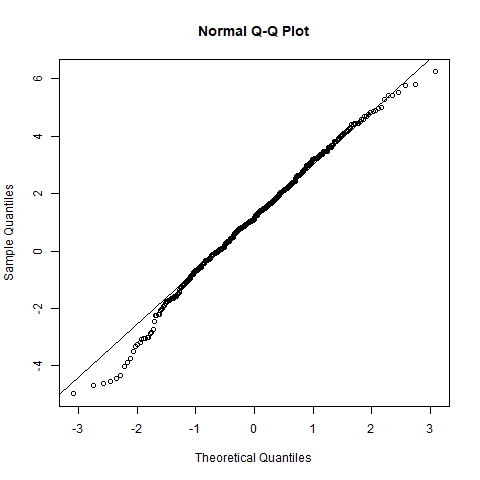
\includegraphics[width=10cm]{../data/img/Salt_Lake_Diff_QQ_Plot.PNG}
  \caption{Q-Q Plot in Salt Lake City}
  \label{fig:slc_diff_qqplot}
\end{figure}

\begin{figure}
  \centering
  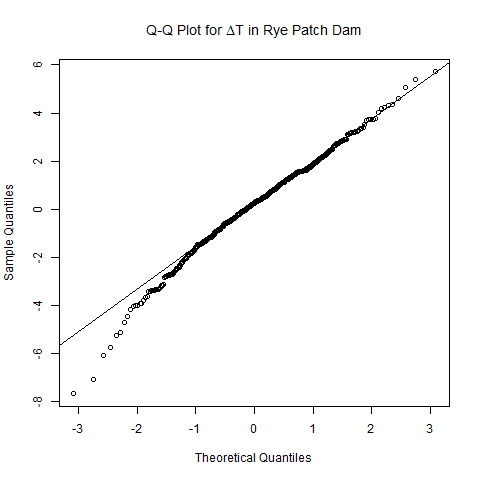
\includegraphics[width=10cm]{../data/img/Rye_Patch_Diff_QQ_Plot.PNG}
  \caption{Q-Q Plot in Rye Patch}
  \label{fig:rp_diff_qqplot}
\end{figure}

We then randomly selected 10\% of the data from each station to remove from the dataset and treat as missing. Although our dataset contains ample missing values on its own, we removed more values in order to evalued the effects of missing data. Our analysis ignored months in which temperature data for Salt Lake City \textit{or} Rye Patch Dam was missing. This resulted in a loss of total data points greater than 10\%, leaving us with a new sample size (that is different for each run) for each station. Performing the Shapiro-Wilk test again, the distribution of the observations were still normal. The new test statistic for a sample run was -13.984, which is less than the critical value  $-t_{n-1,\alpha/2} = -1.648$ (where n = 397). The p-value was $2.2 \times 10^{-16}$, which is less than the significance level $\alpha = 0.05$ (note that the reported p-value is the same as before because the true value is below machine precision). Therefore, we reject $H_{0}$ and conclude that the mean temperature anomaly at Salt Lake City is greater than the mean temperature anomaly at Rye Patch Dam. The addition of more missing values reduced the sample size and (theoretically) resulted in a higher p-value, but did not change the outcome of the hypothesis test.

\section{Second Hypothesis}
The second hypothesis analyzes which environmental factors are the best predictors of temperature in Salt Lake City. According to the EPA, higher temperature results in either more or less precipitation and higher frequency of storms\cite{epa_utah}. This study performs a multiple linear regression of temperature against minutes of sunlight, number of days with thunderstorms, and precipitation per month. In conjuction with the EPA article noted above, we also considered two key characteristics when deciding which parameters we would include in our study: 

\begin{itemize}
	\item linear relationship with temperature, and
	\item availability of data.
\end{itemize}

For example, we did not include total monthly snowfall or number of days with fog because they have too much missing data despite having a decent linear relationship. The parameter with the most significant linear relationship with temperature is, not suprisingly, minutes of sunlight. A major factor we had to consider here, however, was that sunlight data is only recorded from 1965 to 2004. Thus, in order to include this parameter in our analysis, we needed to restrict our study down to this range (roughly 479 total months, or observations). Additionally, we limited the data used in our study to months for which the data was available for all four parameters listed above. Therefore, when including temperature, precipitation, and number of thunderstorms in our study, our sample size decreased from 479 months to 321 months because at least one of the these parameters was missing data in the 479 months of data avialable between 1965 and 2004.

For each parameter identified above, we graphically examine its relation with temperature via a scatter plot with a line of best fit. As expected, there is a strong positive correlation between minutes of sunlight and temperature, as seen in Figure \ref{fig:temp_vs_sun}. Similarly, albeit not as strong, there also appears to be a positive correlation between number of days with thunderstorms and temperature, as seen in Figure \ref{fig:temp_vs_dthunderstorms}. Lastly, the correlation between precipitation and temperature is negative, as seen in Figure \ref{fig:temp_vs_precipitation}, which is expected in some regions as stated by the EPA \cite{epa_utah}.

As an additional preliminarly analysis, in order to obtain a strong multiple linear regression model to estimate temperature, we sought to use parameters that are not highly correlated with each other, as including additional variables that are highly correlated is more likely to simply increase model complexity as opposed to improve the model fit. Figure \ref{fig:correlation_plot}, which is a correlation matrix of the three independent parameters, suggests that the independent variables of sunlight, days with thunderstorms, and precipitation are not highly correlated, further supporting our decision to include them as parameters in our model.

At this point, we conducted the analysis on the selected paramters. Per Table \ref{tab:lin_regression}, we can see the the model has an adjusted $R^{2}$ of $0.7969 \approx$ 0.8, meaning that roughly 80.0\% of the variance in temperature can be explained by the three predictors. Using the coefficients from the table, we can estimate temperature as $\hat{T} = \beta_{0} + X_{1}\beta_{1} + X_{2}\beta_{2} + X_{3}\beta_{3}$, where indices 1, 2, and 3 reference minutes of sun, days with thunderstorms, and precipitation, respectively. Substituting $\beta$ values from Table \ref{tab:lin_regression}, $$\hat{T} \approx -5.26 + 1.04 \times 10^{-3}X_{1} + 0.84X_{2} - 4.80\times 10^{-2}X_{3}.$$

Now that we have completed our multiple linear regression analysis on the three selected parameters, we turn to a final model comparison analysis. Here, we conduct a best subset analysis to locate the best model at each model size, including 1, 2, and 3 parameters. The best subset selection process considers all $3 \choose k$ possibilities, where k is the number of parameters (k = 1, 2, 3). For each k, the best subset method will select the model with the lowest SSE. As can been seen in Table \ref{tab:optimal_selection}, the best models for k = 1, 2, and 3 are minutes of sun, minutes of sun + days with thunderstorms, and minutes of sun + days with thunderstorms + percipitation, respectively.

Now that we have our three best models at each k, we will calculate the following metrics for each model: 

\begin{itemize}
	\item adjusted $R^{2}$,
	\item AIC, and
	\item BIC.
\end{itemize}

The adjusted $R^{2}$ will measure what percentage of the variance in the model is explained by the parameters; this measure penalizes model complexity relative to $R^{2}$. Akaike Information Criterion (AIC) and Bayesian Information Criterion (BIC) are both penalized-likelihood criteria, where the BIC penalizes model complexity a bit more than AIC. Overall, the best model of the three from Table \ref{tab:optimal_selection} will have the greatest adjusted $R^{2}$ and the lowest AIC and BIC values. Define: 

\begin{itemize}
	\item Model 1: Performs a regression against minutes of sunlight
	\item Model 2: Performs a regression against minutes of sunlight + days with thunderstorms
	\item Model 3: Performs a regression against minutes of sunlight + days with thunderstorms + precipitation
\end{itemize} 

Table \ref{tab:model_info} contains these values for each model. The full model, model 3, is the best overall model to choose to estimate temperature because it has the highest adjusted $R^{2}$ and lowest AIC and BIC values.

To demonstrate our results, let us consider the following example to predict the average monthly temperature of a new observation $Y^{*}$. Notationally, the following formula enables the calculation of an $(1-\alpha)$-level prediction interval for $Y^{*}$. $$Y^{*} \pm \hat{Y}^{*} + t_{n-(k+1),\alpha/2} s \sqrt{1+\textbf{x}^{*T}\textbf{V}\textbf{x}^{*}}$$ where $\hat{Y}^{*}$ is the estimate of $Y^{*}$, $t_{n-(k+1),\alpha/2}$ is the critical value, n is the number of observations (n = 321), k is the number of predictors (k = 3), $s$ is the estimate for $\sigma$, equivalent to $\sqrt{MSE}$, $\textbf{x}^{*}$ is the predictor variables for the three parameters, and $\textbf{V} = (\textbf{X}^{T}\textbf{X})^{-1}$, where $\textbf{X}$ represents the matrix of the values of the predictor variables \cite{tamhane}.

Now, given a new month with 15,000 minutes of sunlight, 4 days with thunderstorms, and 35 millimeters of total precipitation, we can calculcate a 95\% prediction interval. To avoid extrapolation, the parameter figures above are all within the ranges of values observed for each parameter in the 321 oberservations analyzed. Utilizing the prediction interval with 95\% confidence, the average monthly temperature of this new month would be between $4.48^{\circ}$C and $19.63^{\circ}$C (with $\hat{Y}^{*} = 12.06^{\circ}$C).

To investigate the effects of missing data on the multiple linear regression, we removed 5\% of temperature observations, 5\% of sunlight observations, 5\% of thunderstorm observations, and 5\% of precipitation observations. We then ignored any data point for which at least one of these four observations was missing, resulting in a smaller sample size. Because of the random nature of the removal of data, the new sample size is approximately 80\% of the original sample size for each run. The new adjusted $R^{2}$ is $0.797 \approx 0.8$, indicating that roughly 80\% of the variation in temperature can be explained by the three predictors. This is not appreciably different from the adjusted $R^{2}$ for the full data set from 1965 to 2004, which was also approximately 80\%. The new estimate for temperature is $$\hat{T} \approx -4.79 + 1.03 \times 10^{-3}X_{1} + 0.85X_{2} - 6.30\times 10^{-2}X_{3}.$$ See Table \ref{tab:lin_regression_missing_data} for the $\beta$ values and p-values for all three predictor variables in the missing data case. Table \ref{tab:model_info_missing_data} implies that Model 3 is once again optimal.


\section{Missing Data}
When data are missing at random, the value of the missing data is not related to the reason for its missingness. In this case, the complete data points are essentially a random sample of the entire dataset, so missing points can be ignored in the analysis. We evaluated the effects of data missing at random on our hypothesis test and multiple linear regression in sections 2 and 3 respectively.

Missing data is non-ignorable if the value of the missing data is related to the reason for its missingness. For example, a storm could cause data collection equipment to become inoperable, and the storm data would not be collected. In this case, it is not possible to ignore the missing data in the analysis because the complete data is no longer a random sample, and therefore does not represent the whole of the data. The Heckman correction is a method that can correct bias from this non-random sample\cite{mnar}. In the context of regression, suppose we want to fit the linear model $$Y_{i} = X_{i}\beta+\epsilon$$ to our data. Heckman's model lets us obtain unbiased estimators of $\beta$. First, we introduce the selection equation $P(R_{yi} = 1 | X_{i}^{s}) = \Phi(X_{i}^{s}\beta^{s})$, where $R_{yi}$ is an indicator variable equal to $1$ if $Y_{i}$ is observed and $0$ if $Y_{i}$ is missing. We use maximum likelihood estimation, a method of estimating parameters by maximizing the likelihood function, to find estimates for $\hat{\beta}^{s}$. Using these estimates, we can compute the inverse Mills ratio $\hat{\lambda}_{i} = \frac{\phi(X_{i}^{s}\hat{\beta}^{s})}{\Phi(X_{i}^{s}\hat{\beta}^{s})}$ for each observation in the sample, where $\phi$ is the standard normal density and $\Phi$ is the standard normal distribution function. Finally, using the linear equation $Y_{i} = X_{i}\beta + \hat{\lambda}_{i}\beta_{\lambda} + \eta_{i}$, where $\eta \sim \mathcal{N}(0,\sigma_{\eta}^{2})$, we can find estimators for $\hat{\beta}$ and $\hat{\beta}_{\lambda}$. There also exists a one-step procedure for estimating $\beta$ which generates a lower standard error, but the two-step procedure is used for faster computation.

After obtaining our estimates for $\beta$, we can draw $\sigma_{\eta}^{2*}$, $\beta^{*}$, and $\beta_{\lambda}^{*}$ from the linear equation. Also, we can draw $\eta^{*}$ from $\mathcal{N}(0,\sigma_{\eta}^{2*})$. Finally, for each missing $Y$, we can impute $$Y_{i}^{*} = X_{i}\beta^{*} + \frac{-\phi(\widehat{X_{i}^{s}\beta^{s})}}{1-\Phi(\widehat{X_{i}^{s}\beta^{s}})}\beta_{\lambda i}^{*}+\eta^{*}.$$

\section{R Code Compilation Instructions}
To run the R scripts, it is imperative to do so from the /data subdirectory as both reference data from a relative path. The team ran the scripts from Terminal with the "Rscript" command instead of RStudio; they could possibly be run from RStudio, but we did not test it with this. 

If not installed already, one can install the libraries used by the scripts by entering the following commands in Terminal:

\begin{itemize}
	\item R
	\item $>$install.packages("ggpubr")
	\item $>$install.packages("ggplot2")
	\item $>$install.packages("latex2exp")
	\item $>$install.packages("car")
	\item $>$install.packages("corrplot")
	\item $>$install.packages("leaps")
\end{itemize}

One can run the scripts by executing the following commands in Terminal:

\begin{itemize}
	\item cd $<$Base Directory$>$/AMS\_572\_Project/data
	\item Rscript Hypothesis\_1.R
	\item Rscript Hypothesis\_2.R
\end{itemize}

% Put references, in BibTeX format, in the file refs.bib
\bibliographystyle{siamplain}
\bibliography{refs}

\section{Appendix: Tables and Figures}
\newpage
\begin{table}[ht]
 \begin{centering}
 \begin{tabular}{|c|c c|} 
 \hline
 $$ & $\Delta Temp$ Salt Lake City & $\Delta Temp$ Rye Patch \\ [0.5ex] 
 \hline\hline
  $\mu$ & 1.1229 & 0.1317 \\ 
 \hline
 $\sigma$ & 1.9765 & 1.9226 \\
  \hline
 $n$ & 487 & 487 \\ 
  \hline
 $P_{Shapiro}$ & 0.0166 & 0.0003 \\ 
 \hline
 \end{tabular}
 \caption{Temperature Difference Statistics}
 \label{tab:temp_diffs}
 \end{centering}
\end{table}

\begin{table}[ht]
 \begin{centering}
 \begin{tabular}{|c|c|} 
  \hline
  Parameter & Value \\
  \hline\hline
  $t$ & -16.46 \\ 
 \hline
 $df$ & 486 \\
  \hline
 $P$ & $2.2 \times 10^{-16}$ \\ 
  \hline
 Conf. Interval & $(-1.1095, -0.8728)$ \\ 
 \hline
 \end{tabular}
 \caption{Paired t Test Results for Temperature Difference}
 \label{tab:t_test_results}
 \end{centering}
\end{table}

\begin{figure}
  \centering
  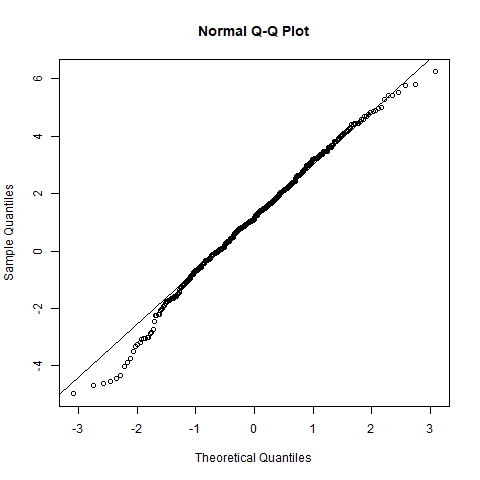
\includegraphics[width=7cm]{../data/img/Salt_Lake_Diff_QQ_Plot.PNG}
  \caption{Q-Q Plot in Salt Lake City}
  \label{fig:slc_diff_qqplot}
\end{figure}

\begin{figure}
  \centering
  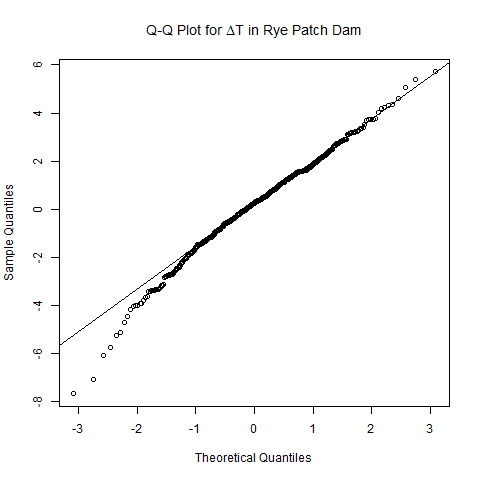
\includegraphics[width=7cm]{../data/img/Rye_Patch_Diff_QQ_Plot.PNG}
  \caption{Q-Q Plot in Rye Patch}
  \label{fig:rp_diff_qqplot}
\end{figure}

\begin{table}[ht]
 \begin{centering}
 \begin{tabular}{|c|c c|} 
 \hline
 $$ & $\Delta Temp$ Salt Lake City & $\Delta Temp$ Rye Patch \\ [0.5ex] 
 \hline\hline
  $\mu$ & 1.1282 & 0.1457 \\ 
 \hline
 $\sigma$ & 1.9850 & 1.9051 \\
  \hline
 $n$ & 390 & 390 \\ 
  \hline
 $P_{Shapiro}$ & 0.0238 & 0.0005 \\ 
 \hline
 \end{tabular}
 \caption{Temperature Difference Statistics for Missing Values}
 \label{tab:temp_diffs_missing}
 \end{centering}
\end{table}

\begin{table}[ht]
 \begin{centering}
 \begin{tabular}{|c|c|} 
  \hline
  Parameter & Value \\
  \hline\hline
  $t$ & -15.03 \\ 
 \hline
 $df$ & 389 \\
  \hline
 $P$ & $2.2 \times 10^{-16}$ \\ 
  \hline
 Conf. Interval & $(-1.1109, -0.8539)$ \\ 
 \hline
 \end{tabular}
 \caption{Paired t Test Results for Temperature Difference for Missing Values}
 \label{tab:t_test_results_missing}
 \end{centering}
\end{table}

\begin{figure}
  \centering
  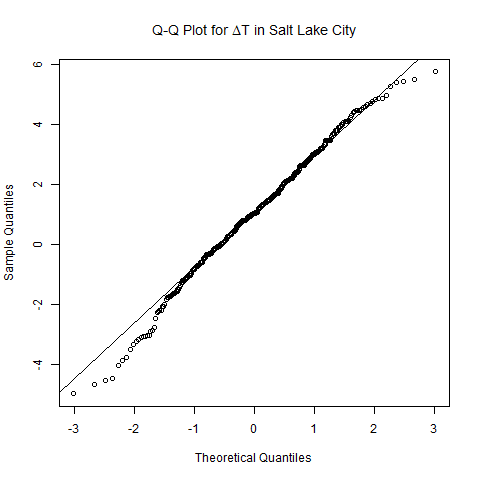
\includegraphics[width=7cm]{../data/img/Salt_Lake_Diff_QQ_Plot_missing_data.png}
  \caption{Q-Q Plot in Salt Lake City with 10\% missing data}
  \label{fig:slc_diff_qqplot_missing}
\end{figure}

\begin{figure}
  \centering
  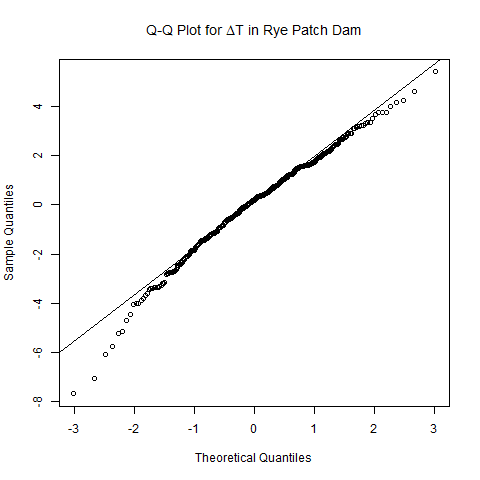
\includegraphics[width=7cm]{../data/img/Rye_Patch_Diff_QQ_Plot_missing_data.png}
  \caption{Q-Q Plot in Rye Patch with 10\% missing data}
  \label{fig:rp_diff_qqplot_missing}
\end{figure}
\begin{figure}
  \centering
  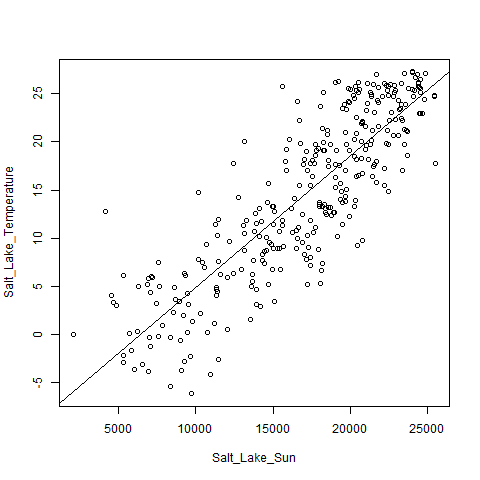
\includegraphics[width=7cm]{../data/img/Temp_vs_sun.PNG}
  \caption{Salt Lake City Temperature versus Sun}
  \label{fig:temp_vs_sun}
\end{figure}

\begin{figure}
  \centering
  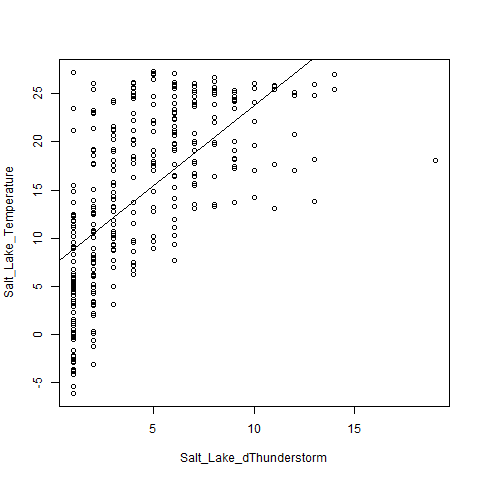
\includegraphics[width=7cm]{../data/img/Temp_vs_dThunderstorm.PNG}
  \caption{Salt Lake City Temperature versus Days of Thunderstorms}
  \label{fig:temp_vs_dthunderstorms}
\end{figure}

\begin{figure}
  \centering
  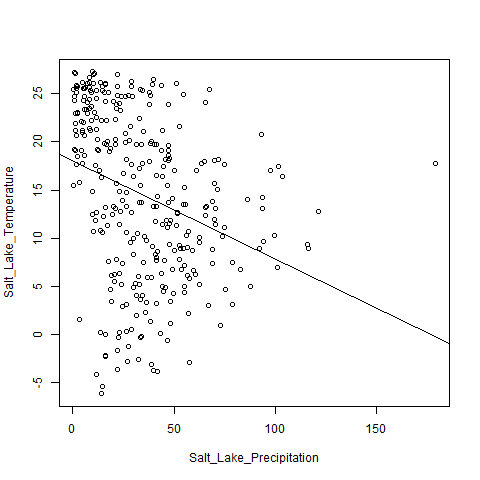
\includegraphics[width=7cm]{../data/img/Temp_vs_Precipitation.PNG}
  \caption{Salt Lake City Temperature versus Precipation}
  \label{fig:temp_vs_precipation}
\end{figure}

\begin{figure}
  \centering
  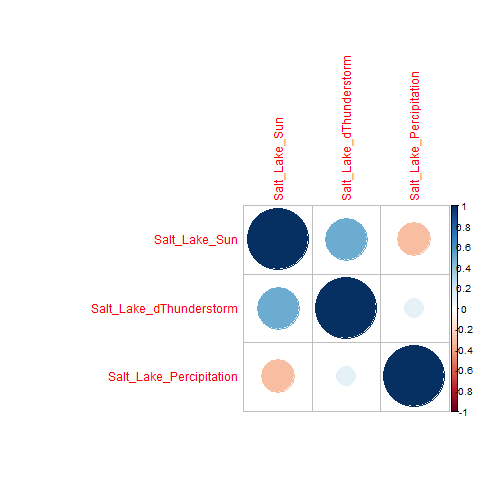
\includegraphics[width=7cm]{../data/img/correlation_plot.PNG}
  \caption{Correlation plot of chosen dependent variables}
  \label{fig:correlation_plot}
\end{figure}

\begin{table}[ht]
 \begin{centering}
 \begin{tabular}{|c|c c c c c|} 
 \hline
 $$ & & & & Days of & \\ [0.5ex] 
 & Temperature & Intercept & Minutes of Sun & Thunderstorms & Precipitation \\
 \hline\hline
 $P_{Shapiro}$ & $2.662\times 10^{-8}$ & -- & $6.845\times 10^{-9}$ & $9.438\times 10^{-15}$ & $2.817\times 10^{-12}$ \\ 
 \hline
 $\beta$ & -- & -5.261 & $1.041\times 10^{-3}$ & 0.8471 & $-4.800\times 10^{-2}$ \\ 
 \hline
 $P(>|t|)$ & -- & $2.30\times 10^{-8}$ & $< 2.00\times 10^{-16}$ & $< 2.00\times 10^{-16}$ & $< 2.91\times 10^{-7}$ \\ 
 \hline
 \end{tabular}
 \caption{Multilinear Regression for Predicting Temperature (Adjusted $R^{2} = 0.7969$, $n = 321$)}
 \label{tab:lin_regression}
 \end{centering}
\end{table}

\begin{table}[ht]
 \begin{centering}
 \begin{tabular}{|c|c c c|} 
 \hline
  \# Variables & Minutes of Sun & Days of Thunderstorms & Precipitation \\
 \hline
 1 & * & & \\
  \hline
 2 & * & * & \\ 
  \hline
 3 & * & * & *\\ 
 \hline
 \end{tabular}
 \caption{Optimal Subset selection for Multilinear Regression}
 \label{tab:optimal_selection}
 \end{centering}
\end{table}

\end{document}
